\chapter{Ingewonnen informatie}
\label{cha:bijlage_C}

\section{Elektra prijzen}

\subsection{Accu prijzen}
\vspace{\baselineskip}

\textbf{Specificaties, \cite{Conrad}}\\

Model: \textbf{Black-Decker-PS130-A9252}\\
Voltage:	12 V	\\
Afmetingen:	92 x 81 x 102 mm \\
Kleur:	zwart	\\
Type:	Ni-MH \\
Capaciteit:	2.100 mAh \\
\vspace{\baselineskip}

Model: \textbf{UltraCell-UCG9-12-Deep-Cycle-Gel} \\
Voltage:	12 V	\\
Afmetingen:	151 x 65 x 99 mm \\
Capaciteit:	9.000 mAh	\\
Type:	Sealed Lead Acid - AGM \\
\vspace{\baselineskip}

Model:  \textbf{Associated-NS300D37C006} \\
Voltage:	7,2 V	\\
Type:	Ni-MH\\
Capaciteit:	3.000 mAh	\\
Output connector:	standard tamiya \\
Afmetingen:	130 x 46 x 24 mm \\

\subsection{Elektromotor prijzen}
\vspace{\baselineskip}

\textbf{Specificaties, \cite{Conrad}}
\vspace{\baselineskip}

Model: \textbf{Joy-it Stappenmotor NEMA-17-01 NEMA-17-01 0.4} \\
Voedingsspanning	2.8 V \\
Hoek	1.8 °\\
Moment bij stand	0.4 Nm \\
Max. fasestroom	1.68 A \\
As-Ø	5 mm \\
Aslengte	22 mm \\
Fabrikantnr.	NEMA-17-01 \\
Type	NEMA-17-01 \\
Breedte	47 mm \\
Nominale spanning	2.8 V \\
\vspace{\baselineskip}

Model: \textbf{Joy-it Stappenmotor 0.15 Nm 0.75 mA As-diameter} \\
Hoek	1,8 ° \\
Moment bij stand	0.15 Nm \\
As-Ø	4,5 mm \\
Aslengte	16 mm \\
Breedte	35 mm \\
Nominale stroom	0.75 mA \\
Nominale spanning	4.35 V \\
Fasen	2 \\
As-Ø	4.5 mm \\
Motorlengte	35 mm \\
\vspace{\baselineskip}

Model: \textbf{Brushed universele elektromotor Igarashi N2738-48GF.} \\
Onbelast toerental	16000 omw/min \\
Afgiftevermogen	17 W \\
Voedingsspanning	3 - 9 V/DC \\
Nullast-stroom	0,6 A \\
Belast toerental	13600 omw/min \\
Fabrikantnr.	2738-048-GFC-3 \\
Max. draaimoment	12 Nmm \\
Gem. stroomverbruik	3.5 A \\
Efficiëntie	68 % \\
Aslengte	37.8 mm \\
\vspace{\baselineskip}

\section{Bestaande mechanismes met dezelfde functie.}
\vspace{\baselineskip}

IDA Motor Controller: \\
The IDA motor controller consists of two printed-circuit boards located in the lower Payload Electronics Box (PEB) and provides power conditioning, motor voltage control and drivers, grapple heater drivers, joint encoder counting, and analog-to-digital conversion of potentiometer voltages, temperature sensor voltages, motor currents, and heater current. The PEB provides the interface to the Lander Command and Data Handling (C \& DH) computer over a serial link. Firmware running on the IDA motor controller microprocessor provides for low-level motor command execution to move the joints to the specified positions, grapple heater command execution, analog-to-digital calibration, and sensor monitoring. \cite{r.g._bonitz_nguyen_kim_bonitz_folkner_golombek_olson_spohn_grott_et_al._1970}
\vspace{\baselineskip}

\section{Mogelijke stuursystemen.}
\vspace{\baselineskip}

\begin{figure}[H]
    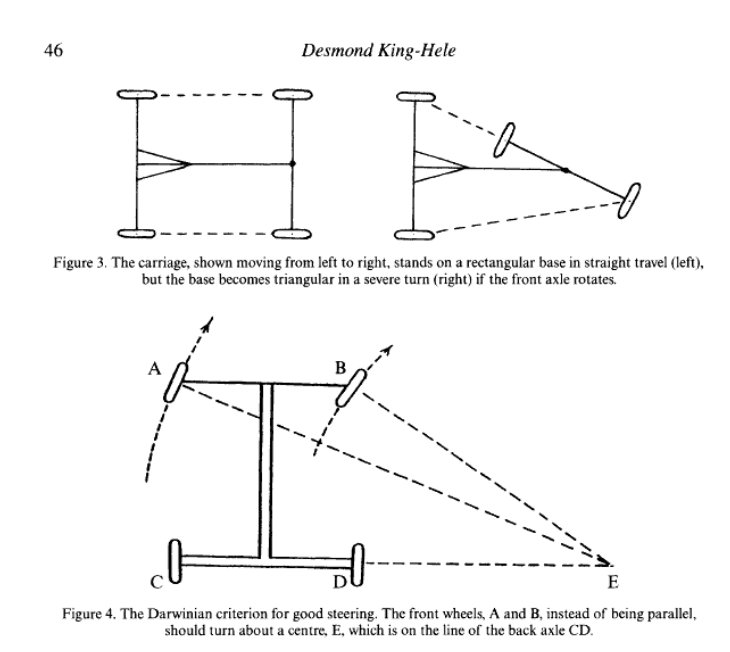
\includegraphics[width=100mm]{06_bijlage_C/ackermann.PNG}
    \caption{Stuursysteem, \cite{king-hele_2002}}
    \label{fig:conceptscores9}
\end{figure}

\vspace{\baselineskip}

\begin{figure}[H]
    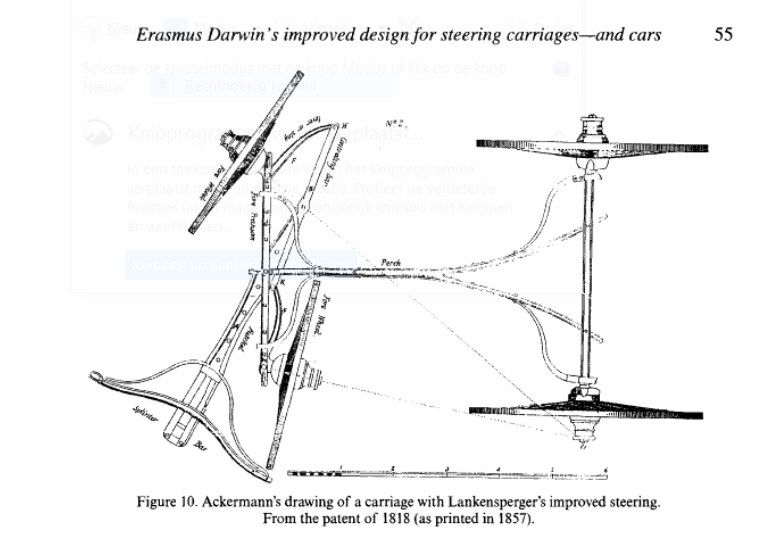
\includegraphics[width=100mm]{06_bijlage_C/Ackermann2.PNG}
    \caption{Stuursysteem, \cite{king-hele_2002}}
    \label{fig:conceptscores0}
\end{figure}
